
%%%%%%%%%%%%%%%%%%%%%%% file typeinst.tex %%%%%%%%%%%%%%%%%%%%%%%%%
%
% This is the LaTeX source for the instructions to authors using
% the LaTeX document class 'llncs.cls' for contributions to
% the Lecture Notes in Computer Sciences series.
% http://www.springer.com/lncs       Springer Heidelberg 2006/05/04
%
% It may be used as a template for your own input - copy it
% to a new file with a new name and use it as the basis
% for your article.
%
% NB: the document class 'llncs' has its own and detailed documentation, see
% ftp://ftp.springer.de/data/pubftp/pub/tex/latex/llncs/latex2e/llncsdoc.pdf
%
%%%%%%%%%%%%%%%%%%%%%%%%%%%%%%%%%%%%%%%%%%%%%%%%%%%%%%%%%%%%%%%%%%%


\documentclass[runningheads,a4paper]{llncs}

\usepackage{amssymb}
\setcounter{tocdepth}{3}
\usepackage{graphicx}
\usepackage{subfigure}
\usepackage{url}
\urldef{\mails}\path{Corresponding_email: xiejuany@snnu.edu.cn}
%\urldef{\mailsb}\path|hcgao,|
%\urldef{\mailsc}\path| }@snnu.edu.cn|    
\newcommand{\keywords}[1]{\par\addvspace\baselineskip
\noindent\keywordname\enspace\ignorespaces#1}

\begin{document}

\mainmatter  % start of an individual contribution

% first the title is needed
\title{A stable gene subset selection algorithm for cancers}

% a short form should be given in case it is too long for the running head
\titlerunning{A stable gene subset selection algorithm}

% the name(s) of the author(s) follow(s) next
%
% NB: Chinese authors should write their first names(s) in front of
% their surnames. This ensures that the names appear correctly in
% the running heads and the author index.
%
\author{Juanying Xie%
%\thanks{Please note that Juanying Xie is the corresponding author of the paper.}%
\thanks{Corresponding author: Juanying Xie. Email: xiejuany@snnu.edu.cn}
\and Hongchao Gao  }
%
\authorrunning{Juanying Xie and Hongchao Gao}
% (feature abused for this document to repeat the title also on left hand pages)

% the affiliations are given next; don't give your e-mail address
% unless you accept that it will be published
\institute{School of Computer Science, Shaanxi Normal University, Xi'an,710062, PR China\\
%Tiergartenstr. 17, 69121 Heidelberg, Germany\\
\mails\\
%\mailsa\\
%\mailsb\\
%\mailsc\\
%\url{http://www.springer.com/lncs}
}

%
% NB: a more complex sample for affiliations and the mapping to the
% corresponding authors can be found in the file "llncs.dem"
% (search for the string "\mainmatter" where a contribution starts).
% "llncs.dem" accompanies the document class "llncs.cls".
%

%\toctitle{Lecture Notes in Computer Science}
%\tocauthor{Authors' Instructions}
\maketitle


\begin{abstract}
In order to solve the problem that the selected genes are depend on the train subset in the gene subset selection algorithms, we propose an assemble method to select the discrimination genes for cancers, so that a stable gene subset can be obtained. We randomly extract some proportional samples from train subset and cluster the genes of these samples in K-means, then select a typical gene from each cluster according to its weight estimated in Pearson correlation coefficient between genes and labels. This process is repeated several times. Those genes with high frequencies in the processes are selected to construct the selected gene subset. The power of the proposed method is tested on three very popular gene datasets, and the experimental results demonstrate that the new algorithm proposed in this paper has found the most stable gene subset with the highest classification accuracy.
\keywords{gene selection\enspace\enspace gene subsets\enspace\enspace K-means\enspace\enspace assemble\enspace\enspace Pearson correlation coefficient\enspace\enspace cancers}
\end{abstract}


\section{Introduction}

With the development of DNA microarray technology, there are more and more gene expression datasets with tens of thousands of genes and small numbers of samples. To analyze this kind of dataset, the first important thing is to reduce the dimensionality of it, that is to search and find those genes which can distinguish samples from different classes \cite{ding2005minimum,guyon2003introduction,guyon2002gene}. Therefore there are more and more experts focus on this field, and there are lots of gene selection algorithms being emerged \cite{bermejo2011grasp,sasikala2014multi,lu2012novel}. However, the available gene selection algorithms cannot guarantee that the gene subset they found is stable. Many of them have got the disadvantages that the gene subset is variant with the different train subset from the same gene expression dataset. The worst case is that there is no one common gene in any two gene subsets. However, in bioinformatics area, especially for the medical doctors they usually want to find the specific and stable genes in which they can tell patients from normal people. Therefore, to find the stable gene subset has become an urgent issue in gene selection  area. 

It is well know that K-means \cite{macqueen1967some} is a very fast and simple clustering algorithm, and it can be used to cluster big data \cite{huang1998extensions}. So we adopts K-means to cluster genes into clusters, where the genes in a same cluster are very similar, and the ones in different clusters are dissimilar to each other. Then we select one typical gene from one cluster to construct the gene subset. We have demonstrated the correctness of the clustering based gene selection idea in \cite{xjy2014}. However, the clustering result of K-means is depend on the initial centers, which caused the unstable in the gene subset. Furthermore, the variance of train subset on which the K-means runs accelerates the unstable of the selected gene subset. How to find the stable gene subset with high classification accuracy is a challenging problem in gene selection study \cite{han2012variance,yu2012stable,yu2008stable}.

In order to solve the aforementioned problem, this paper proposes an assemble method for selecting the discrimination genes of cancers, so that a stable gene subset can be obtained. We run K-means several times to get several gene subsets, then we  merge the gene subsets and select the genes with high frequencies. We test the power of the new gene subset selection algorithm on three popular gene datasets. The experimental results proved that the new gene subset selection algorithm can find the most stable gene subset with highest classification accuracy compared to the famous gene subset selection algorithms, such as MRMR and SVM-RFE.

The paper is organized as follows: Section 2 introduces our proposed new gene subset selection algorithm in detail. Section 3 tests our proposed gene selection algorithm on three popular gene datasets, and compares its performance with MRMR and SVM-RFE in terms of the classification accuracy, variance and gene iteration rate. Section 4 draws some conclusions.

\section{The proposed gene subset selection algorithm}
We adopt K-means to cluster genes, so that the similar genes are grouped into same cluster and the dissimilar genes are in different clusters.  Then a typical gene is selected from one cluster, and the genes from each cluster comprise a gene subset.

\subsection{The importance of genes to classification}

There are many metrics to evaluate the importance of a gene to classification, such as Relief-F, information gain, t-test and Wilcoxon Signed-rank test $et~al$ \cite{guyon2002gene,xjy2014}. We use Pearson correlation coefficient in equation (\ref{eqn:PCC}) to assess the importance of a gene to classification. 

\begin{equation}\label{eqn:PCC}
R(i) = \frac{ \sum\limits_{k=1}^{n}(x_{k,i}-\bar{x}_i)(y_k-\bar{y})}{\sqrt{\sum\limits_{k=1}^{n}(x_{k,j}-\bar{x}_i)^2(y_k-\bar{y})^2}}
\end{equation}

where $n$ is the total number of samples in a gene dataset, $R(i)$ means the importance of the $ith$ gene to the classification, $x_{k,i}$  is the value of the $ith$ gene in the $kth$ sample, $\bar{x}_{i}$  is the mean value of the $ith$ gene, $y_k,~\bar{y}$ are respectively the label of the $kth$ sample and the mean of the labels for all samples in a gene dataset. 

It can be seen from the equation (\ref{eqn:PCC}) that $R(i)\in [-1,1]$ , where $R(i)=1$ means the $ith$ gene is positive correlation to the label, and $R(i)= -1$ means the negative correlation between the $ith$ gene and the label. The value of $|R(i)|$ varies from 0 to 1, and the higher the value of  $|R(i)|$, the more importance is the $ith$ gene to classification. When $|R(i)|=1$ holds, the $ith$ gene can tell patients from normal people correctly.

\subsection{The way to partition a dataset and to estimate the power of a gene subset}

It is known that the selected gene subset may vary with the partition of a gene dataset. In order to reduce the influence of a dataset partition on the selected gene subset, we adopt bootstrap \cite{han2006data} to partition a gene dataset into train subset and test subset.

The different train subset may lead to the different selected gene subset, so we repeat our algorithm 50 times to get the statistical result of it. We calculate the classification accuracy of the selected gene subset in equation (\ref{eqn:ACC}) \cite{han2006data}, where $M$ is the classification model built on the selected gene subset. The average classification accuracy of 50 runs of each algorithm is compared.

\begin{equation}\label{eqn:ACC}
Acc = 0.632\times{Acc(M)_{test\_subset}} + 0.368\times{Acc(M)_{train\_subset}}
\end{equation}

%
%\begin{equation}\label{eqn:ACC}
%Acc = \sum\limits_{i=1}^{T}0.632\times{Acc(M_i)_{test\_subset}} + 0.368\times{Acc(M_i)_{train\_subset}}
%\end{equation}


\subsection{The description of our algorithm}

We partition a gene dataset into train subset and test subset in bootstrap \cite{han2006data}, then we randomly extract samples from the train subset in proportion of 80\%, and run K-means algorithm on the extracted samples to group similar genes into same clusters and dissimilar genes into different clusters. Then choose one typical gene from each cluster to construct a gene subset. This process is repeated 20 times, so we get 20 gene subsets. We choose genes with high frequencies in the 20 gene subsets to comprise the selected gene subset, and evaluate the property of the selected gene subset to classification in equation (\ref{eqn:ACC}).



Here are the detail steps of our algorithm.


\textbf{Input:} $Data = \{ x_i \}_{i=1}^n$, cluster number $K$ for K-means, parameter $\gamma$ for K-means repeating times, parameter $\varphi$  for the proportion to extract samples from train subset, parameter $\tau$ for the number of genes  in the selected gene subset.

\textbf{Output:} the selected gene subset and its classification accuracy.
 
\emph {step} 1:~data preprocessing, fill the missing values and normalize data;

\emph{step} 2:~partition dataset into $train\_subset$ and $test\_subset$, let $|train\_subset| = T$  and $cr = 1$ ;
 
\emph{step} 3:~randomly extract samples from $train\_subset$ in proportion~$\varphi$, that is $T'= \varphi T$ , and use K-means to cluster genes of extracted samples into clusters, and calculate the importance of genes in equation (\ref{eqn:PCC}) using the extracted samples; 
 
\emph{step} 4:~select the most important gene from each cluster to comprise a gene subset $S$;

\emph{step} 5:~save $S$ to $TS$, let $cr = cr + 1$ , if $cr$ $\prec$ $\gamma$ , then go to \emph{step} 3;

\emph{step} 6:~select the top $\tau$  genes with high frequencies from $TS$ to construct the selected gene subset, then build a classification model on the selected gene subset, and calculate its classification accuracy in equation (\ref{eqn:ACC}). 


\section{Experimental results and their analysis}
Experiments are conducted on three popular gene datasets including Leukemia \cite{golub1999molecular} and Colon \cite{alon1999broad} and Carcinoma \cite{notterman2001transcriptional}. Table 1 describes the datasets. All the data are normalized in equation (\ref{eqn:normalization}).

\begin{table}\label{tab:data}
\centering
\caption{Description of gene datasets}
\begin{tabular}{cccc}
\hline
Gene datasets & Source	&  Number of genes &	Number of samples\\
\hline
Leukemia & Golub, $et~al$ \cite{golub1999molecular}	&7 129&	72 (47+25)\\
Colon&	Alon, $et~al$ \cite{alon1999broad}&	2 000&	62 (40+22)\\
Carcinoma&	Notterman, $et al$ \cite{notterman2001transcriptional}	&   7 458&	36 (18+18)\\
\hline
\end{tabular}
\end{table}

\begin{equation}\label{eqn:normalization}
g_{i,j} = \frac{ g_{i,j}-min(g_j)}{max(g_j)-min(g_j)}
\end{equation}

where $g_{i,j}$  is the value of the gene $j$  in sample $i$, and $min(g_j)$  is the minimum value of gene $j$ , and $max(g_j)$  is the maximum value of gene $j$.

We respectively adopt KNN \cite{cover1967nearest} and SVM \cite{vapnik2000nature} as classification tools. The power of our algorithm proposed in this paper is compared with that of the popular gene subset selection algorithms including  MRMR (minimum redundancy maximum relevance) \cite{ding2005minimum} and SVM-RFE \cite{guyon2002gene}. As a comparison we compared the performance of our algorithm with that of which K-means is executed only once on the whole train subset to select the gene subset. We named our algorithm as \emph{S-Weight} and the other one with only once K-means execution as \emph{Weight}. All the algorithms are respectively repeated 50 times and their average classification accuracy, variance of the classification accuracy and the gene iteration rate \cite{ding2005minimum} of the selected gene subsets are compared. 

The gene iteration rate of two successive selected gene subsets is computed in equation (\ref{eqn:iteration}), where $\tau$ is the size of the selected gene subset, that is, the number of genes in the selected gene subset, and $T$ is the times of each algorithm being repeated. In our experiments the $T$ equals 50. We calculate the gene iteration rate of the selected gene subsets in equation (\ref{eqn:aveiteration}) to assess the stable of the selected gene sunsets by each algorithm.


\begin{equation}\label{eqn:iteration}
IRate_i = \frac{ Subset_i \cap Subset_{i+1} } {\tau},~~~~i = 1, 2, \cdots, T-1
\end{equation}

\begin{equation}\label{eqn:aveiteration}
Iteration\_rat= \frac{1}{T-1}\sum\limits_{i=1}^{T-1}{IRate_i}
\end{equation}

We use the SVM library in \cite{chang2011libsvm} to conduct our experiments, and let the penalize parameter C for the linear kernel of SVM be 20. KNN is that embedded in MATLAB. The parameter K for KNN is set to be 5. All the codes are developed in MATLAB (version  R2012a), and run on an Intel(R) Core(TM)2 Quad CPU Q9500@2.83GHz 2.83GHz PC with 4GB memory using Windows 7 (32 bit) operating system.

\subsection{The experimental results on Colon}

Fig. 1-3 respectively display the experimental results of algorithms on Colon dataset in term of average classification accuracy of the classifiers built on the selected gene subsets, variance of the classification accuracy, and the average gene iteration rate of the selected gene subsets of 50 runs of the algorithms. Where the subfigures (a) and (b) in Fig. 1-2 respectively display the results of algorithms when the SVM and KNN classifiers are used.

\begin{figure}
\label{fig:fig1}
\centering
\subfigure[]{\label{fig:fig1a}
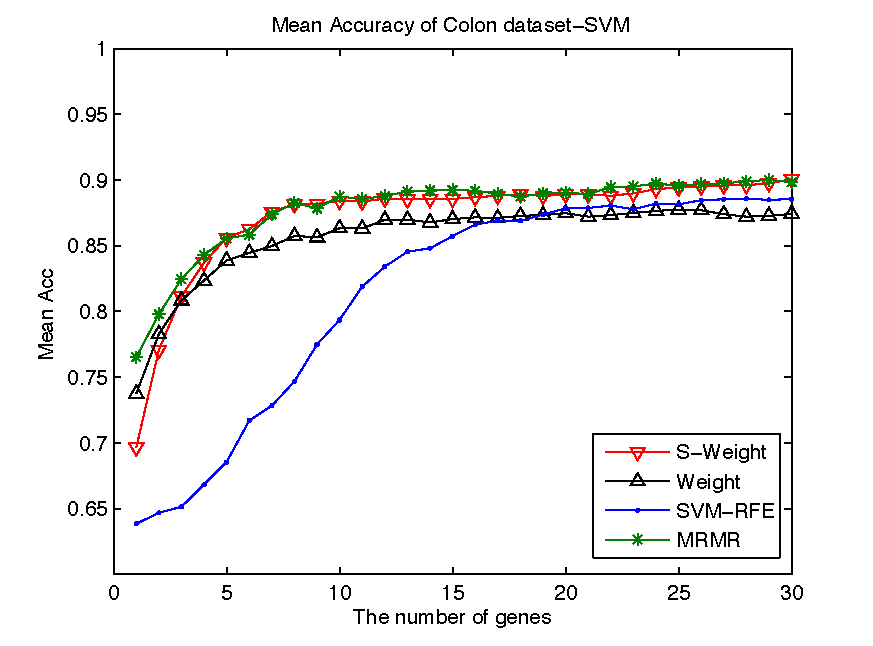
\includegraphics[width=5.5cm]{fig1a.pdf}
}
\hspace{0.5cm}
\subfigure[] { \label{fig:fig1b}     
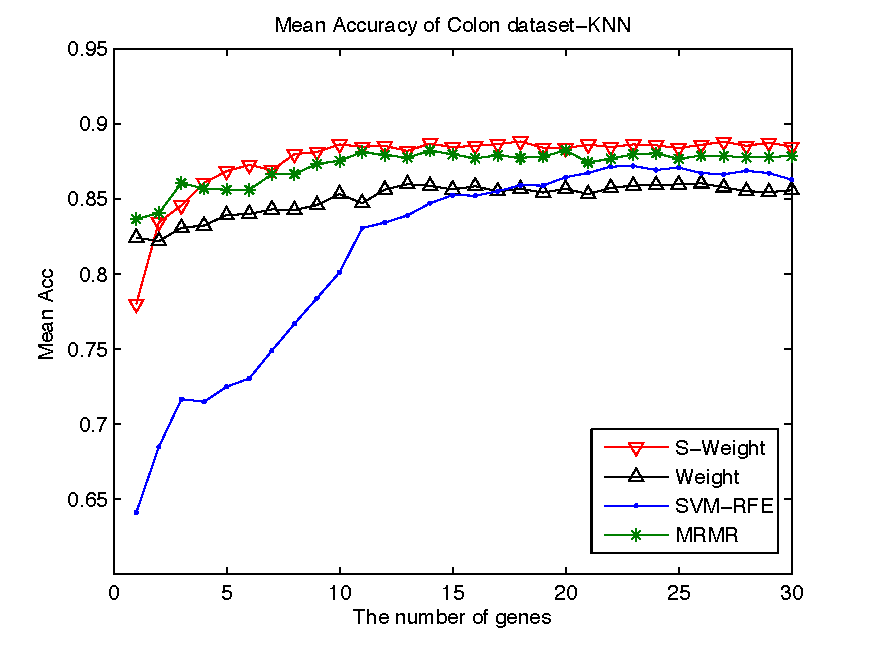
\includegraphics[width=5.5cm]{fig1b.pdf}     
}   
\caption{The average classification accuracy of gene subsets by four algorithms on Colon dataset, (a) SVM, (b) KNN.}
\end{figure}

The results in Fig. 1-(a) reveal that the performance of our proposed S-Weight is similar to that of MRMR, and both of the algorithms outperforms Weight and SVM-RFE. The results in Fig. 1-(b) reveal that our S-Weight algorithm has got the best performance when the KNN classifier is used, followed by MRMR. Both of the results in Fig.1-(a) and Fig. 1-(b) demonstrate that Weight outperformed SVM-RFE when the number of selected genes is less than 15, otherwise it was defeated by SVM-RFE in terms of  mean accuracy no matter the classifier is SVM or KNN. 

\begin{figure}
\label{fig:fig2}
\centering
\subfigure[]{\label{fig:fig1a}
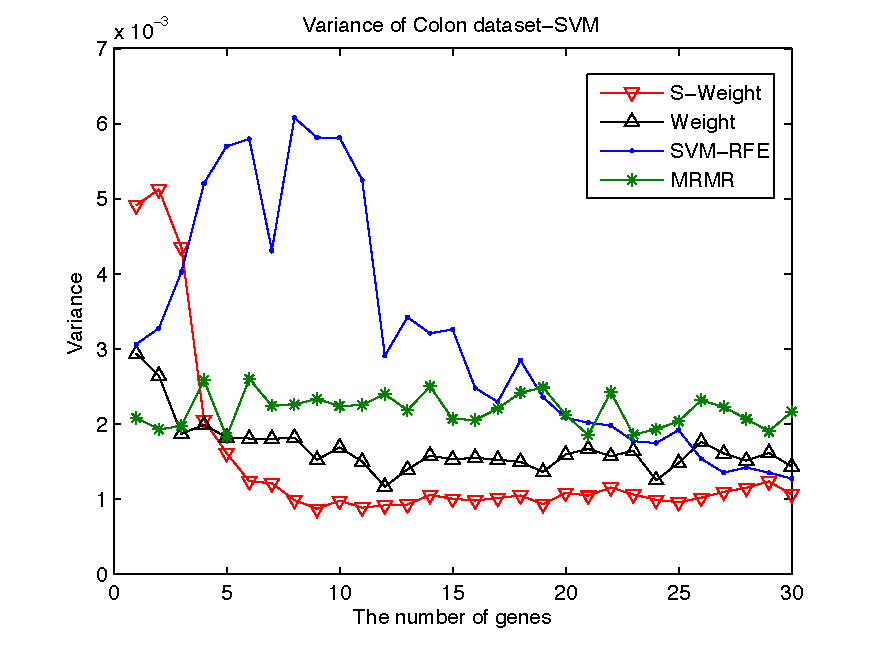
\includegraphics[width=5.5cm]{fig2a.pdf}
}
\hspace{0.5cm}
\subfigure[] { \label{fig:fig1b}     
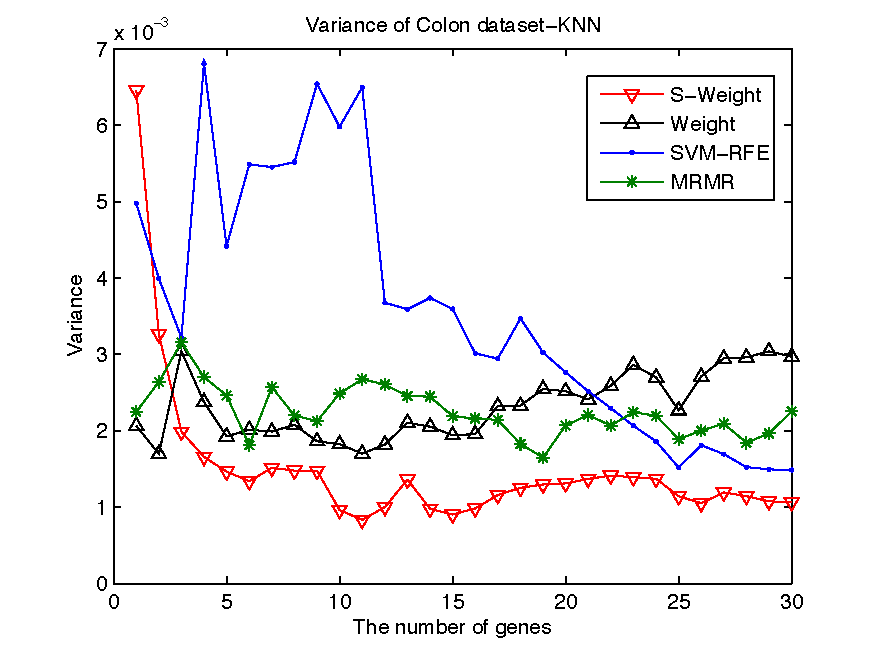
\includegraphics[width=5.5cm]{fig2b.pdf}     
}   
\caption{The variance of classification accuracy of gene subsets by four algorithms on Colon dataset, (a) SVM, (b) KNN.}
\end{figure}

It can be seen from the results in Fig. 2-(a) and Fig. 2-(b) that the variance of the classification accuracy of selected gene subsets by our S-weight has got the minimum value, which means that our S-weight algorithm has found the gene subset with most stable property in classification accuracy. The performance of SVM-RFE in terms of variance is the worst one when the number of selected genes is less than 20. The performance of Weight and MRMR are in the middle place among the compared algorithms with a relative stable variance no matter how many genes are selected and which classifier is used. 

\begin{figure}
\centering    
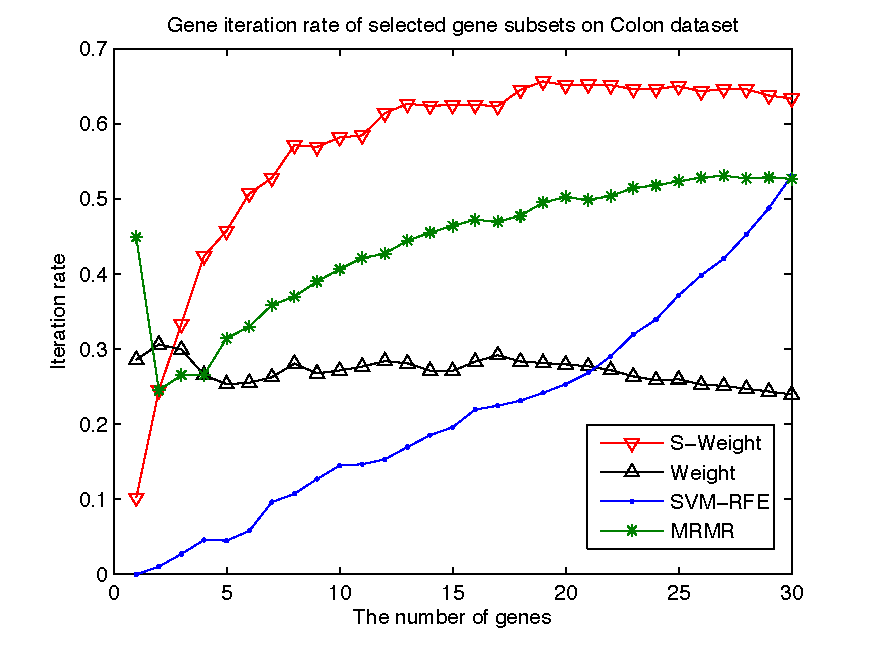
\includegraphics[width=8cm]{fig3.pdf}
\caption{ The gene iteration rate of selected gene subsets by four algorithms of their 50 runs on Colon dataset. }     
\label{fig:fig3}     
\end{figure}

The results in Fig. 3 reveal that there are more than 60\% genes are same in the selected gene subsets by our S-Weight algorithm, followed by MRMR where there are more than 50\% genes are duplicated in the selected gene subsets when the number of selected genes is greater or equal to 20. Weight has found genes with about 25\% overlapping no matter how many genes are selected. The gene iteration rate of the selected gene subsets of SVM-RFE goes up with the number of selected genes. 

The above analysis of four algorithms in terms of gene iteration rate and the variance of classification accuracy of selected gene subset on Colon dataset demonstrates that our S-Weight is the most stable gene subset selection algorithm among the popular gene selection algorithms including SVM-RFE and MRMR, and with the highest classification accuracy as well.


\subsection{The experimental results on ALL/AML Leukemia}

Fig. 4-6 display the experimental results of four algorithms on Leukemia dataset in terms of average classification accuracy, variance of the accuracy and the gene iteration rate of the selected gene subsets. Where the subfigures (a) and (b) of Fig. 4-5 respectively display the results of SVM and KNN classifiers are used.

\begin{figure}
\centering
\subfigure[]{\label{fig:fig4a}
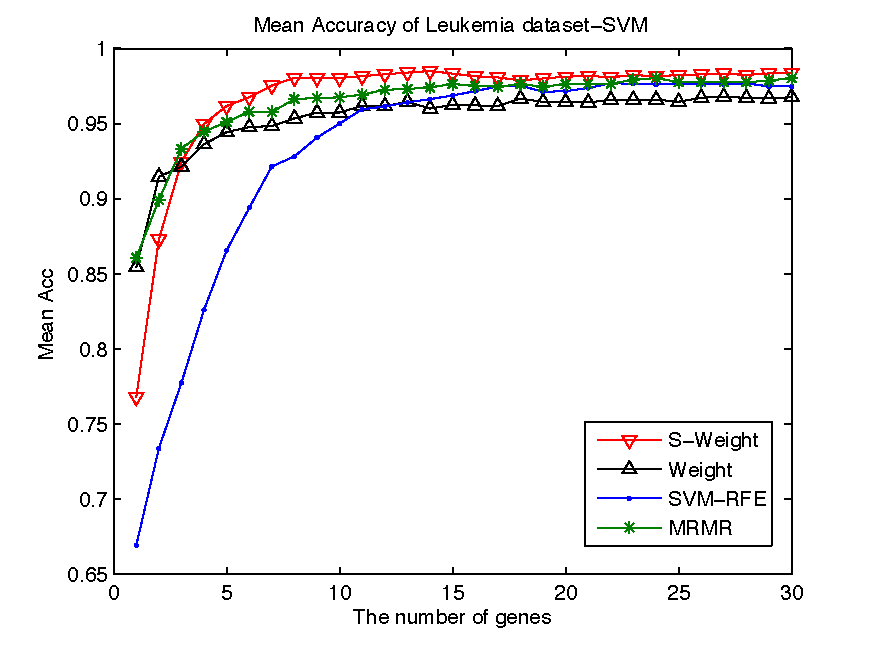
\includegraphics[width=5.5cm]{fig4a.pdf}
}
\hspace{0.5cm}
\subfigure[] { \label{fig:fig4b}     
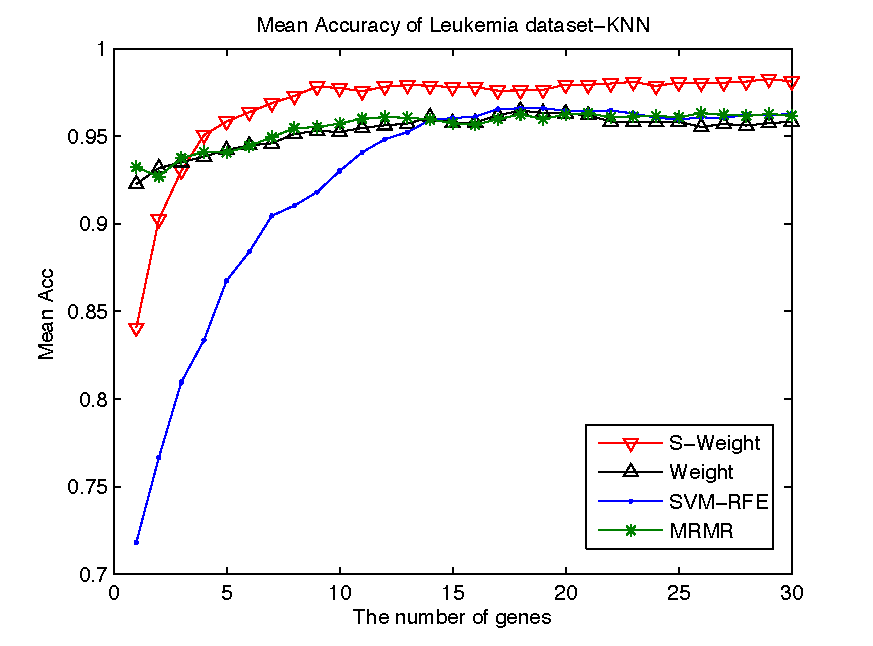
\includegraphics[width=5.5cm]{fig4b.pdf}     
}   
\caption{The average classification accuracy of gene subsets by four algorithms on Leukemia dataset, (a) SVM, (b) KNN.}
\label{fig:fig4}
\end{figure}

From the results shown in Fig. 4-(a) and Fig. 4-(b), we can see that our proposed S-Weight algorithm has obtained the best classification accuracy, especially in Fig. 4-(b) where the KNN classifier is adopted, the performance of our S-Weight is much better than that of the other three algorithms. The results in Fig. 4-(b) still reveal that the Weight and MRMR have got the similar classification power no matter how many genes are there in the selected gene subset when KNN classifier is used. The SVM-RFE has obtained the similar performance with MRMR when there are more than 15 genes being selected, otherwise its performance is the worst when KNN classifier is used. The results in Fig. 4-(a) demonstrate that MRMR has got a little better performance than Weight does when the SVM classifier is used, and the SVM-RFE has obtained a little better performance than Weight when the size of the selected gene subset is greater than 10, otherwise it is the worst one among the four compared gene subset selection algorithms in terms of classification accuracy.

\begin{figure}
\centering
\subfigure[]{\label{fig:fig5a}
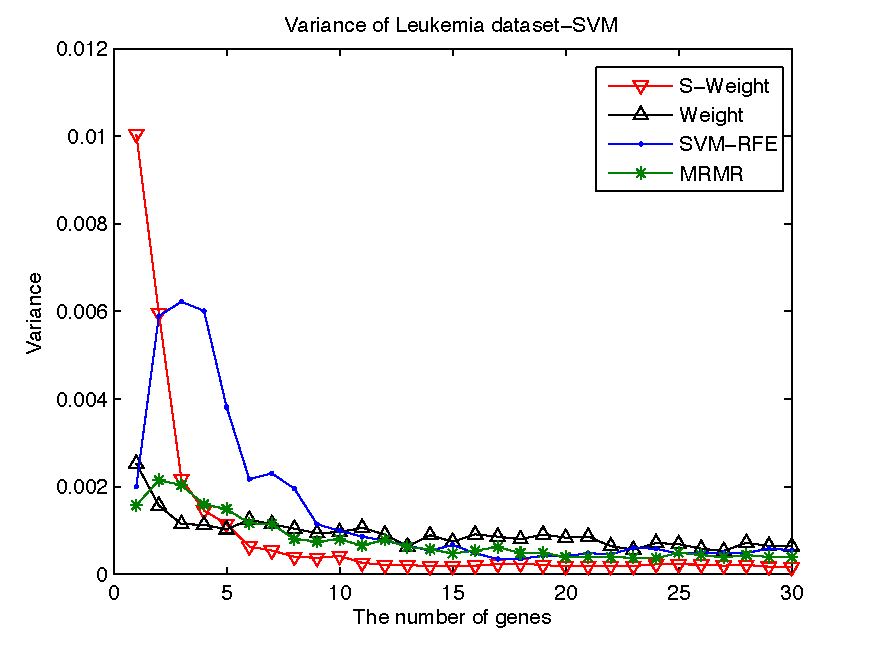
\includegraphics[width=5.5cm]{fig5a.pdf}
}
\hspace{0.5cm}
\subfigure[] { \label{fig:fig5b}     
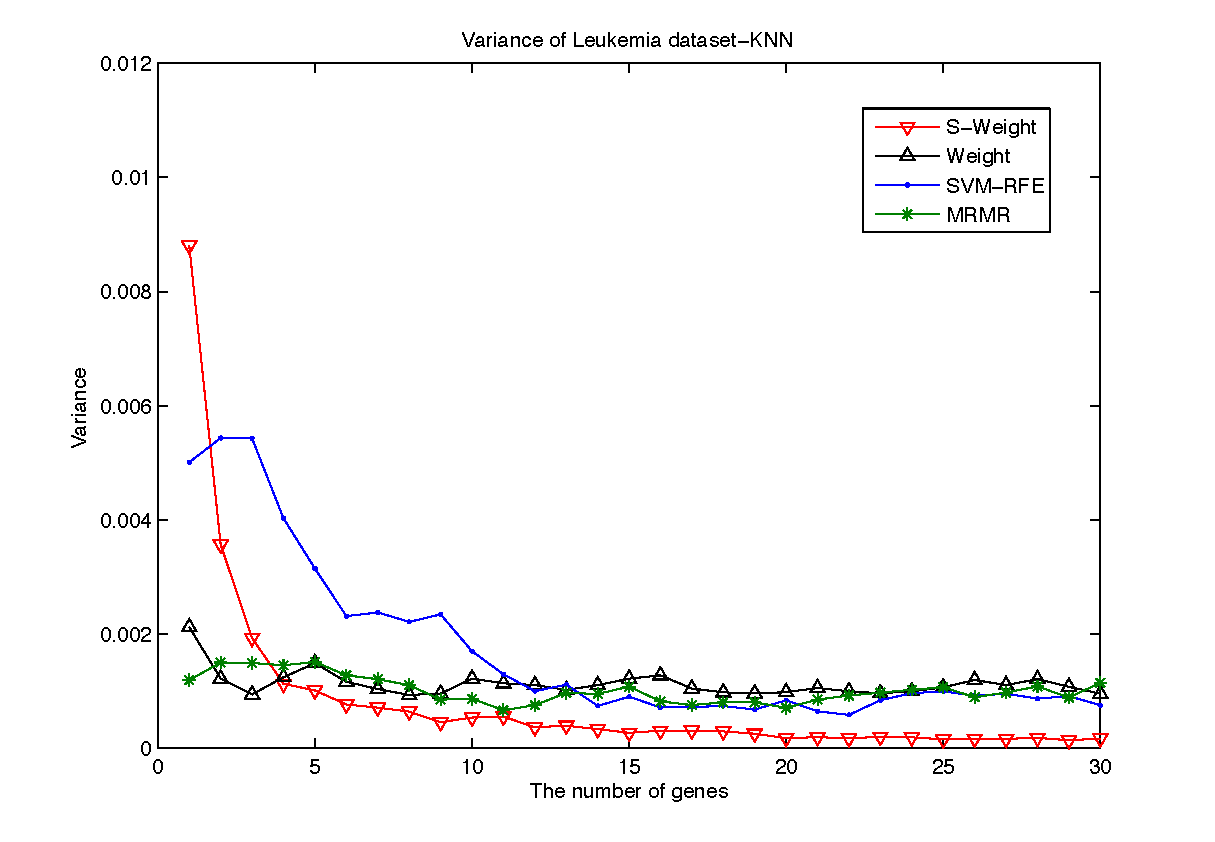
\includegraphics[width=5.5cm]{fig5b.pdf}     
}   
\caption{The variance of classification accuracy of gene subsets by four algorithms on Leukemia dataset, (a) SVM, (b) KNN.}
\label{fig:fig5}
\end{figure}

The experimental results in Fig. 5 reveal that the proposed S-weight algorithm has found the gene subsets on which we can build a classifier with minimum variance of classification accuracy. The performance of SVM-RFE in terms of variance is the worst one when the number of selected genes is less than 10. The performance of Weight and MRMR are similar with a relative stable variance no matter how many genes are selected and which classifier is adopted.

\begin{figure} 
\centering    
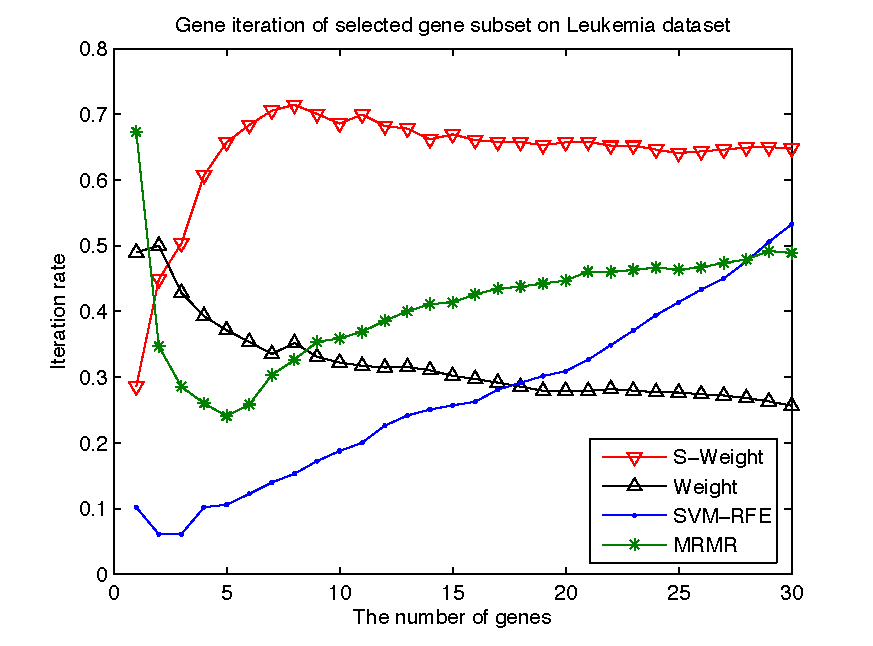
\includegraphics[width=8cm]{fig6.pdf}
\caption{ The gene iteration rate of selected gene subsets by four algorithms on Leukemia dataset. }     
\label{fig:fig6}     
\end{figure}

The experimental results in Fig. 6 show that the gene iteration rate of the selected gene subsets by our S-Weight algorithm is up to 60\% - 70\%, which is much higher than that of other three gene selection algorithms. This means that S-Weight algorithm can find the most stable gene subset. The gene subset by SVM-RFE is the most unstable one whose gene iteration rate goes up with the number of genes in the gene subset. The gene iteration rate of  selected gene subsets by MRMR is higher than  that by Weight when the number of selected genes is more than 10.

\subsection{The experimental results on Carcinoma }
Fig. 7-9 display the experimental results of four algorithms on Carcinoma dataset respectively in term of mean classification accuracy of classifiers on corresponding gene subsets, and the variance of the classification accuracy, and the gene iteration rate of selected gene subsets when the algorithms are repeated 50 times.

\begin{figure}
\centering
\subfigure[]{\label{fig:fig7a}
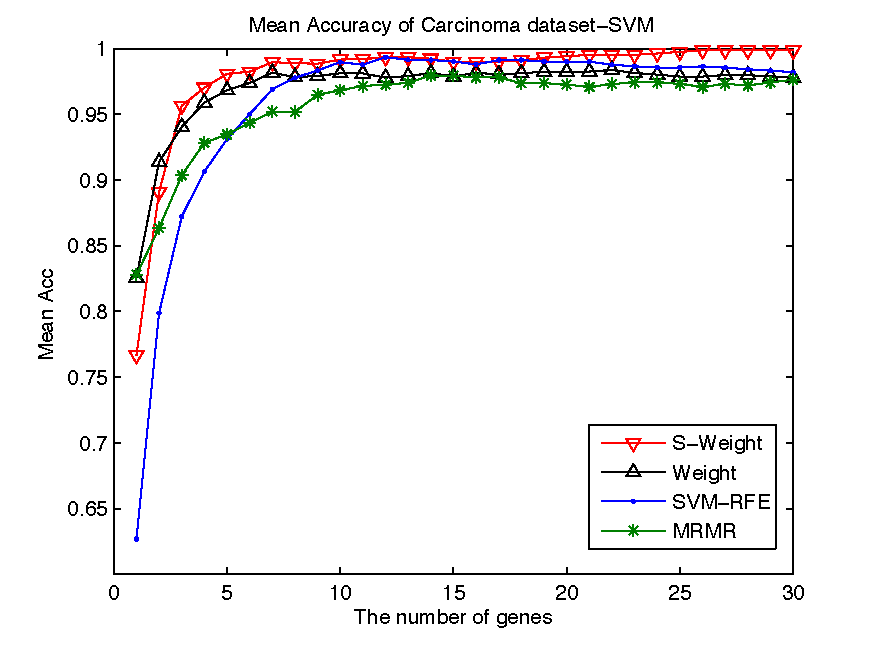
\includegraphics[width=5.5cm]{fig7a.pdf}
}
\hspace{0.5cm}
\subfigure[] { \label{fig:fig7b}     
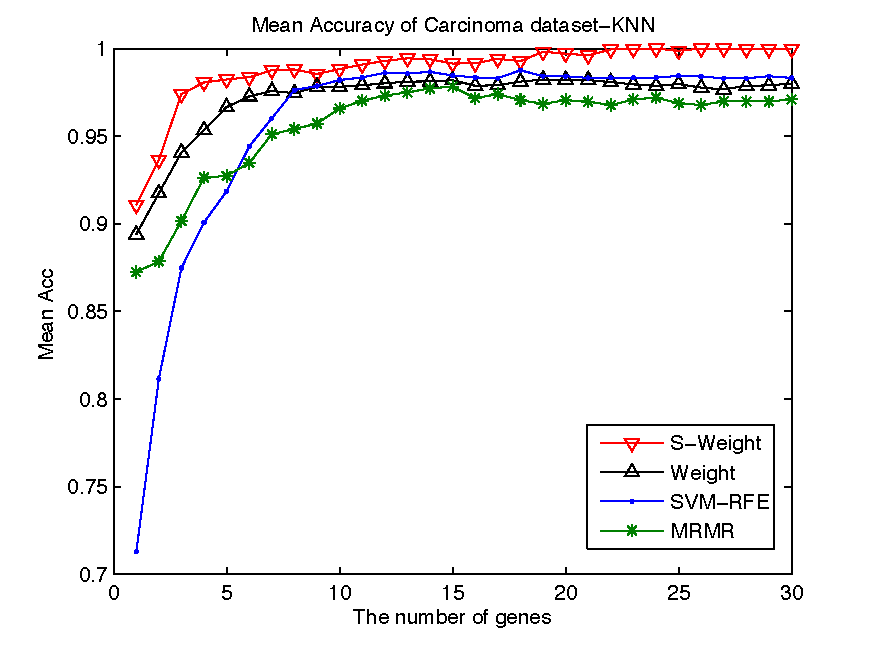
\includegraphics[width=5.5cm]{fig7b.pdf}     
}   
\caption{The average classification accuracy of gene subsets by four algorithms on Carcinoma dataset, (a) SVM, (b) KNN.}
\label{fig:fig7}
\end{figure}

The experiments results in Fig. 7-(a) and Fig. 7-(b) reveal that S-Weight algorithm can found the gene subset with the highest classification accuracy, even up to 100\% when the number of selected gens is up to 20. The other three algorithms have got very similar performance, especially when the number of selected genes is over 15. Although MRMR, SVM-RFE and Weight algorithms are not as good as S-Weight algorithm, they can find gene subsets whose classification accuracy is over 95\% even up to 98\%. 

\begin{figure}[t]
\centering
\subfigure[]{\label{fig:fig8a}
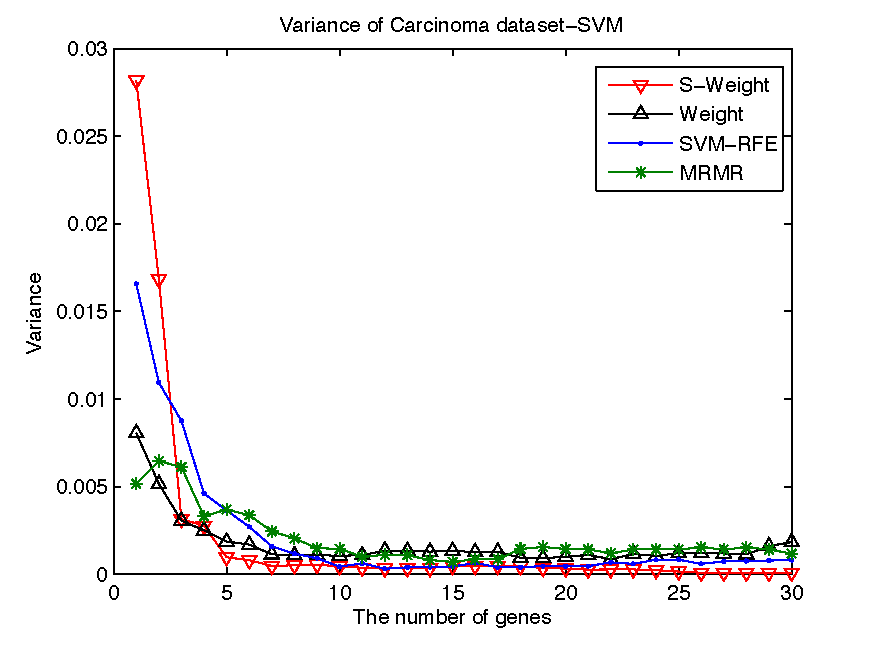
\includegraphics[width=5.5cm]{fig8a.pdf}
}
\hspace{0.5cm}
\subfigure[] { \label{fig:fig8b}     
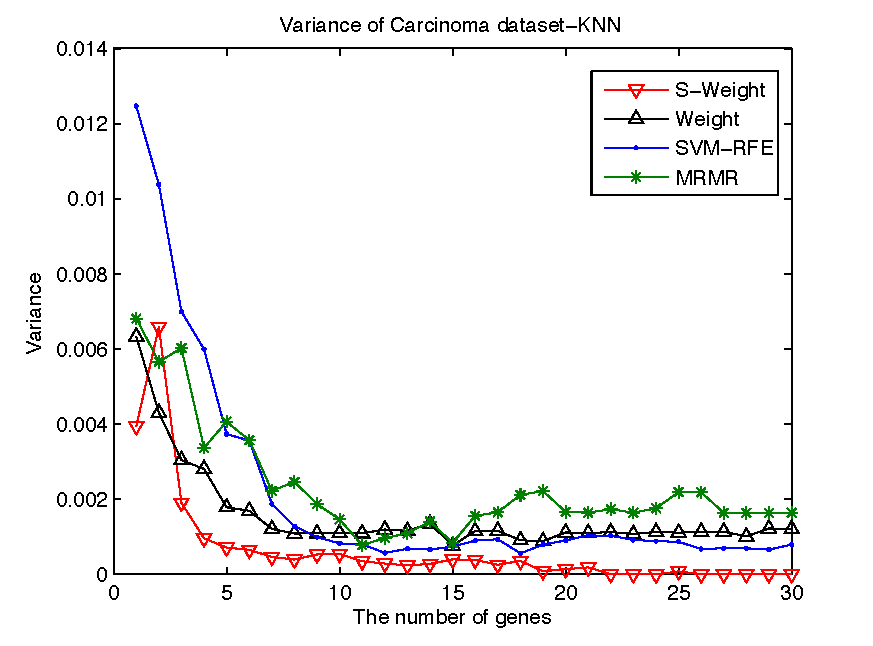
\includegraphics[width=5.5cm]{fig8b.pdf}     
}   
\caption{The variance of classification accuracy of gene subsets by four algorithms on Carcinoma dataset, (a) SVM, (b) KNN.}
\label{fig:fig8}
\end{figure}


The comparison of variance of classification accuracy of selected gene subsets in Fig. 8-(a) and Fig. 8-(b) demonstrates that S-Weight algorithm can find the gene subsets with the lowest variance value. When the number of the selected genes is over 5, the variance of S-Weight reaches 0. Therefore, S-Weight is the best one among the four gene subset selection algorithms. From Fig. 8-(a), it can be seen that SVM-RFE, Weight and MRMR are very similar in terms of variance of the classification accuracy on the selected gene subsets when the SVM classifier is built. The results in Fig. 8-(b) reveal that MRMR is the worst one among the four gene subset selection algorithms when the KNN classifier is used, and SVM-RFE and Weight algorithms are similar to each other.


\begin{figure}
\centering    
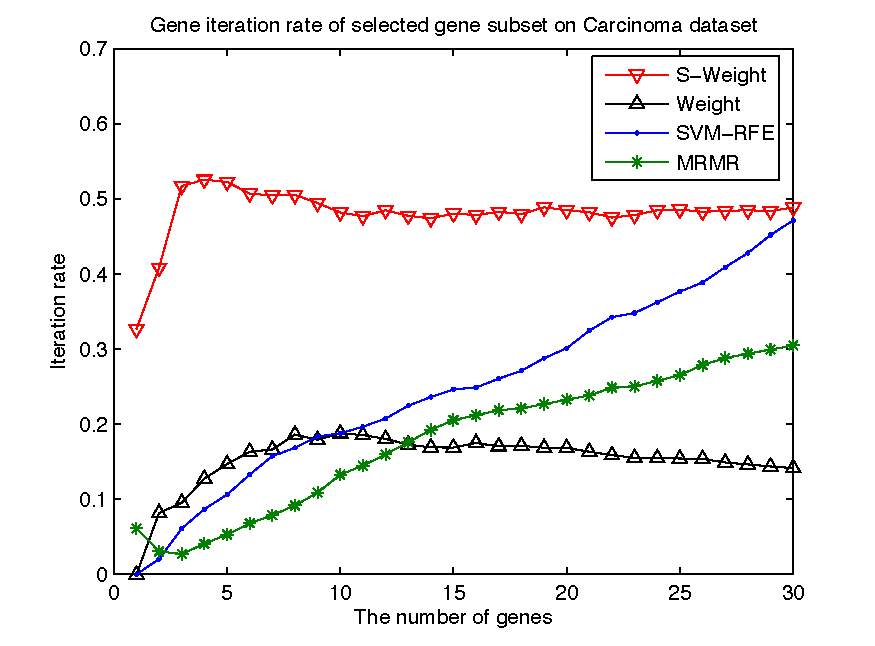
\includegraphics[width=8cm]{fig9.pdf}
\caption{The gene iteration rate of selected gene subsets by four algorithms on Carcinoma dataset. }     
\label{fig:fig9}     
\end{figure}


The experimental results in Fig. 9 show that our S-Weight is the most stable gene subset selection algorithm among the four compared algorithms. There are half genes are same in the selected gene subsets.  The Weight algorithm is the worst one with the lowest gene iteration rate of no more than 20\%. MRMR and SVM-RFE are not stable gene selection algorithms whose gene iteration rate goes up with the number of selected genes in the gene subset, but the upper bound of their gene iteration rate is no more than that of S-Weight. 


\section{Conclusions}

This paper proposes a stable gene subset selection algorithm, named S-Weight. It randomly extracts samples from train subset and clusters the genes of the extracted samples in K-means, and estimates the importance of each gene of the extracted samples in Pearson correlation as well. Then it selects the most important gene from each cluster to construct the gene subset with K genes. This process is repeated several times, and the genes with high frequency will be selected to construct the selected gene subset. 

The power of S-Weight is tested on three popular gene expression datasets, and compared with that of the famous gene selection algorithms including MRMR and SVM-RFE, and with that of Weigh algorithm which is the special case of S-weight where K-means is executed only once on the whole train subset to select the top K important genes to comprise the selected gene subset. The performances of the algorithms are compared in term of the classification accuracy of classifiers built on the selected gene subset, variance of the classification accuracy, and the gene iteration rate. All experimental results demonstrate that our proposed S-Weight algorithm can find the most stable gene subset with high classification accuracy. It outperforms MRMR and SVM-RFE and Weight. 

It can be concluded that our S-weight to some extent has solved the exiting problem in gene selection area that the selected gene subset varies with the train subset.


\subsubsection*{Acknowledgments.}
We are much obliged to those who provide the public gene datasets for us to use. This work is supported in part by the National Natural Science Foundation of China under Grant No. 31372250, is also supported by the Key Science and Technology Program of Shaanxi Province of China under Grant No. 2013K12-03-24, and is at the same time supported by the Fundamental Research Funds for the Central Universities under Grant No. GK201503067..



%\begin{thebibliography}{4}

%\bibitem{jour} Smith, T.F., Waterman, M.S.: Identification of Common Molecular
%Subsequences. J. Mol. Biol. 147, 195--197 (1981)

%\bibitem{lncschap} May, P., Ehrlich, H.C., Steinke, T.: ZIB Structure Prediction Pipeline:
%Composing a Complex Biological Workflow through Web Services. In: Nagel,
%W.E., Walter, W.V., Lehner, W. (eds.) Euro-Par 2006. LNCS, vol. 4128,
%pp. 1148--1158. Springer, Heidelberg (2006)

%\bibitem{book} Foster, I., Kesselman, C.: The Grid: Blueprint for a New Computing
%Infrastructure. Morgan Kaufmann, San Francisco (1999)

%\bibitem{proceeding1} Czajkowski, K., Fitzgerald, S., Foster, I., Kesselman, C.: Grid
%Information Services for Distributed Resource Sharing. In: 10th IEEE
%International Symposium on High Performance Distributed Computing, pp.
%181--184. IEEE Press, New York (2001)

%\bibitem{proceeding2} Foster, I., Kesselman, C., Nick, J., Tuecke, S.: The Physiology of the
%Grid: an Open Grid Services Architecture for Distributed Systems
%Integration. Technical report, Global Grid Forum (2002)

%\bibitem{url} National Center for Biotechnology Information, \url{http://www.ncbi.nlm.nih.gov}

%\end{thebibliography}

\bibliographystyle{llncs}
\bibliography{refs}

%
%\section*{Appendix: Springer-Author Discount}
%
%LNCS authors are entitled to a 33.3\% discount off all Springer
%publications. Before placing an order, the author should send an email, 
%giving full details of his or her Springer publication,
%to \url{orders-HD-individuals@springer.com} to obtain a so-called token. This token is a
%number, which must be entered when placing an order via the Internet, in
%order to obtain the discount.
%
%\section{Checklist of Items to be Sent to Volume Editors}
%Here is a checklist of everything the volume editor requires from you:
%
%
%\begin{itemize}
%\settowidth{\leftmargin}{{\Large$\square$}}\advance\leftmargin\labelsep
%\itemsep8pt\relax
%\renewcommand\labelitemi{{\lower1.5pt\hbox{\Large$\square$}}}
%
%\item The final \LaTeX{} source files
%\item A final PDF file
%\item A copyright form, signed by one author on behalf of all of the
%authors of the paper.
%\item A readme giving the name and email address of the
%corresponding author.


\end{document}
